\chapter{Methodology}
\label{chapter:Methodology}

In this section, the general methodology for evaluating the 
accessibility of HTML/CSS code is described. It includes a combination
of automated auditing tools and manual verification. This hybrid approach 
identifies a wide range of accessibility issues, reconciles inconsistencies and guarantees reliable results. 
Figure~\ref{fig:pipeline} provides an overview of the evaluation pipeline, 
from data collection, prompt design to code generation, accessibility and similarity analysis,
and post-processing.
All evaluations are conducted following WCAG 2.1, the most widely 
adopted standard supported by the tools at the time of this thesis.

\begin{figure}
  \centering
  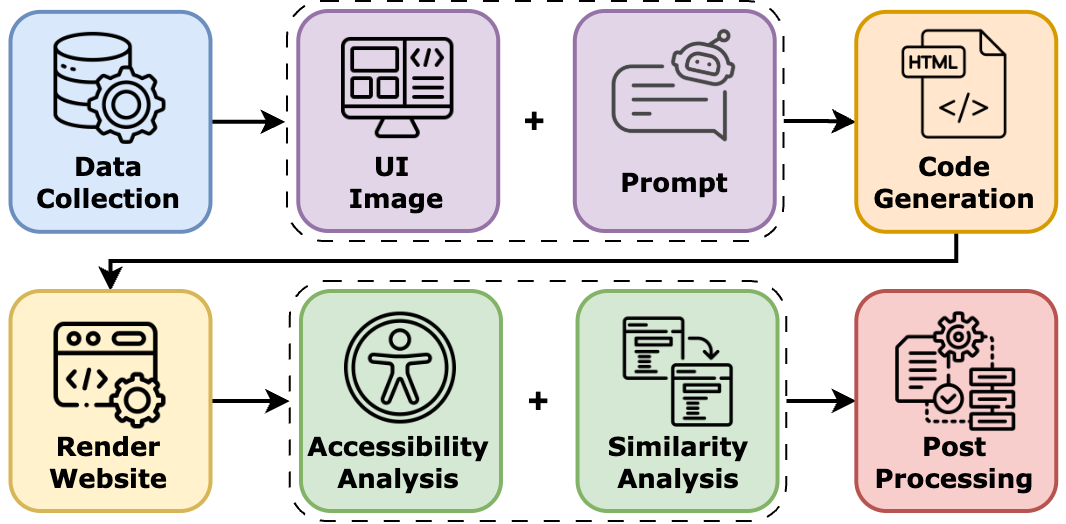
\includegraphics[width=0.5\linewidth]{figures/pipeline_modern.png}
  \caption{Overview of the evaluation pipeline, from data collection and prompt design to code generation, accessibility and similarity analysis, and post-processing.}
  \label{fig:pipeline} 
\end{figure}

\section{Automated Accessibility Evaluation}
A wide range of automated accessibility checkers is available to 
detect violations in web content.
According to former studies, automated testing can detect up to $\sim$60\% 
of accessibility issues~\cite{deque2023accessibility}. This makes them 
valuable for developers; however they can not completely replace manual testing or 
expert review.
Regardless, in practice, a combination of various tools can help minimize the 
oversight of accessibility violations during the tests.\newline
This study uses three widely adopted automated accessibility evaluation 
tools: \textit{Axe-Core}, \textit{Google Lighthouse Accessibility},
and \textit{Pa11y}. Each tool offers unique detection mechanisms,
coverage areas, and reporting formats.
\begin{itemize}
  \item \textbf{Axe-Core (4.10.3)~\cite{web:axecore}:} is a rule-based engine
  developed by Deque Systems and commonly integrated into browser 
  extensions and CI/CD pipelines. It provides detailed information
  and links each violation to its own rule set.
  \item \textbf{Google Lighthouse Accessibility (12.4.0)~\cite{web:lighthouse}:} 
  embedded within Chromium-based browsers, performs accessibility audits
  alongside performance and SEO diagnostics.
  \item \textbf{Pa11y (8.0.0)~\cite{web:pa11y}:} is a flexible command-line tool 
  that uses HTML CodeSniffer as its engine and is especially useful for batch 
  evaluation of static pages. During some tests on the benchmark dataset, 
  it was found that Pa11y has strengths in areas where the other 
  tools seem to fail (e.g., color contrast violations); therefore, it was 
  decided to use it as the third complementary tool.
\end{itemize}
 
\noindent
All three tools were used to evaluate the generated HTML/CSS code. 
However, the outputs of each tool may differ. For example, 
Pa11y flagged a missing label for a form field under WCAG
2.1 Technique F68 (\textit{``This form field should be labelled in some way.''}), 
while Axe-core
reported the same issue using its own rule IDs (e.g. \textit{``label''}) and includes 
WCAG success-criterion
tags such as \textit{``4.1.2 Name, Role, Value''} in the rule metadata, but it does not cite WCAG
techniques. This discrepancy reflects a common challenge in automated accessibility evaluation:
the tools often differ in their interpretation, granularity, and labeling of the same underlying
issues.\newline
To address this inconsistency and improve cross-tool comparability, a 
unified taxonomy of accessibility issues is created. First, all 
detected violations are compiled to 
aggregate the outputs of the three tools. Based on the preserved 
metadata, such as rule IDs, WCAG mappings, descriptions, and affected
HTML elements, the violations are grouped into functionally 
equivalent categories (e.g., missing labels, insufficient color contrast,
missing alt-text). Next, similar rule definitions are combined 
into a single rule, leading to a consistent set of 40 
accessibility categories, each mapped to one or more WCAG 
success criteria. For instance, issues such as \textit{``H43.*''}
(from pa11y) and \textit{``empty-table-header''} (from axe-core) were all
grouped under the category \textit{``Table Headers''}. Similarly,
contrast-related violations were merged
under \textit{``Color Contrast''}, according to WCAG 2.1 1.4.3 Contrast (Minimum), 
regardless of variation in wording across tools.

\subsection{Manual Verification}
As mentioned, automated tools can not completely replace manual testing. 
Certain accessibility guidelines, especially those involving 
contextual understanding or semantic meaning still require 
human judgment. Therefore, we support the evaluation with a 
structured manual review process. During the experiments, the 
generated HTML/CSS is audited manually by using the previously 
created accessibility issue taxonomy, especially identifying 
violations that may be overlooked by automated tools 
(e.g. improper headings, redundant links and semantically 
ambiguous structures). This manual layer of analysis helps 
to provide a more comprehensive and realistic assessment of
the accessibility quality.

\begingroup
    % Spaltentypen, Abstand, Farbe
\newcolumntype{M}{>{\raggedright\arraybackslash}m{2.5cm}}
\newcolumntype{T}{>{\centering\arraybackslash}m{2.0cm}}
\newcolumntype{R}{>{\raggedright\arraybackslash}m{3.4cm}}
\newcolumntype{D}{>{\raggedright\arraybackslash}m{4.58cm}}
\renewcommand{\arraystretch}{1.15}
\definecolor{darkgray}{gray}{.85}

% Makros
\newcommand{\toolsfmt}{Axe-Core/Lighthouse (\textit{Pa11y})}
\newcommand{\rulepair}[2]{#1 (\textit{#2})}

\begin{table}[htbp]
  \tiny\centering
  \begin{tabularx}{\linewidth}{M|T|R|D}
  \hline
  \rowcolor{darkgray}\textbf{VIOLATIONS} & \textbf{TOOLS} & \textbf{RULE ID(S) (TECHNIQUE ID)} & \textbf{DESCRIPTION}\\
  \hline

  % 1) Color Contrast
  Color Contrast
    & \toolsfmt
    & \makecell[l]{\rulepair{color-contrast}{G18, G145}}
    & Text/background contrast below WCAG AA threshold. (SC 1.4.3)\\
  \hline

  % 2) Landmark & Region
  Landmark \& Region
    & \toolsfmt
    & \makecell[l]{%
        \rulepair{landmark-one-main}{–}\\
        \rulepair{landmark-unique}{–}\\
        \rulepair{region}{–}\\
        \rulepair{landmark-no-duplicate-main}{–}\\
        \rulepair{landmark-main-is-top-level}{–}}
    & Landmarks missing, duplicated or incorrectly nested. (SC 1.3.1, 2.4.1)\\
  \hline

  % 3) Label Form Control
  Label Form Control
    & \toolsfmt
    & \makecell[l]{\rulepair{label}{H44, H91, F68}}
    & Form control lacks an accessible label or label text. (SC 1.3.1, 4.1.2)\\
  \hline

  % 4) Headings
  Headings
    & \toolsfmt
    & \makecell[l]{%
        \rulepair{page-has-heading-one}{–}\\
        \rulepair{heading-order}{G141}\\
        \rulepair{empty-heading}{H42, G130}}
    & Headings missing, empty or out of order. (SC 1.3.1, 2.4.6)\\
  \hline

  % 5) Distinguishable Color Links
  Distinguishable Color Links
    & \toolsfmt
    & \makecell[l]{\rulepair{link-in-text-block}{–}}
    & Only colour distinguishes the link from body text. (SC 1.4.1)\\
  \hline

  % 6) Document Language
  Document Language
    & \toolsfmt
    & \makecell[l]{%
        \rulepair{html-has-lang}{H57}\\
        \rulepair{html-lang-valid}{H57, H58}\\
        \rulepair{html-xml-lang-mismatch}{H57, H58}\\
        \rulepair{valid-lang}{H57, H58}}
    & Missing or conflicting page language declaration. (SC 3.1.1, 3.1.2)\\
  \hline

  % 7) Target Size
  Target Size
    & \toolsfmt
    & \makecell[l]{\rulepair{target-size}{–}}
    & Interactive element’s touch target is smaller than WCAG threshold. (SC 2.5.5)\\
  \hline

  % 8) Incomplete Links
  Incomplete Links
    & \toolsfmt
    & \makecell[l]{\rulepair{link-name}{H30, H91.A}}
    & Link has no perceivable name or content. (SC 2.4.4, 2.4.9, 4.1.2)\\
  \hline

  % 9) Image Alt-Text
  Image Alt-Text
    & \toolsfmt
    & \makecell[l]{%
        \rulepair{image-alt}{H36, H67}\\
        \rulepair{input-image-alt}{H37}}
    & Image lacks alternative text. (SC 1.1.1)\\
  \hline

  % 10) Labels of Buttons
  Labels of Buttons
    & \toolsfmt
    & \makecell[l]{%
        \rulepair{input-button-name}{H91}\\
        \rulepair{button-name}{H91}}
    & Button element has no accessible name. (SC 4.1.2)\\
  \hline

  % 11) Table Headers
  Table Headers
    & \toolsfmt
    & \makecell[l]{%
        \rulepair{empty-table-header}{H43}\\
        \rulepair{–}{H63}}
    & Table has missing, empty or incorrect referenced headers. (SC 1.3.1)\\
  \hline

  % 12) Document Title
  Document Title
    & \toolsfmt
    & \makecell[l]{\rulepair{document-title}{H25}}
    & Page \texttt{<title>} element missing or empty. (SC 2.4.2)\\
  \hline

  % 13) Form Submit Button
  Form Submit Button
    & \toolsfmt
    & \makecell[l]{\rulepair{–}{H32}}
    & Form lacks a submit button. (SC 3.2.2)\\
  \hline

  % 14) Duplicate IDs
  Duplicate IDs
    & \toolsfmt
    & \makecell[l]{\rulepair{–}{F77}}
    & Multiple elements share identical \texttt{id} attribute. (SC 4.1.1)\\
  \hline

  % 15) Incorrect List Structure
  Incorrect List Structure
    & \toolsfmt
    & \makecell[l]{%
        \rulepair{list}{H48}\\
        \rulepair{listitem}{H48}}
    & Incorrect list markup (ul/ol/li missing or nested wrongly). (SC 1.3.1)\\
  \hline

  \end{tabularx}
  \caption{Taxonomy of the Top-15 automatically detected accessibility issues and their rule identifiers across the different tools. Axe-Core and Lighthouse report their violations based on the same rule set, while Pa11y uses WCAG techniques as reporting base which are shown in the parentheses.}
  \label{tab:taxonomy}
\end{table}

\endgroup
\newpage

\section{Dataset}
\label{subchapter:Dataset}
\subsection{Scope and Design}
The main goal is to gather a diverse and high-quality dataset which consists of 
paired UI screenshots and HTML/CSS, and represents
real-world webpages. The dataset should (1) include multiple domains and layouts,
(2) contain annotated accessibility violations, and (3) have a reasonable size to be
statistically relevant, but is also small enough to be analyzed manually.
No publicly available dataset fulfills all requirements.

\subsection{Construction}
Two promising examples in the field of Image-to-Code are \textit{Design2Code}~\parencite{si2024design2code} 
and \textit{Webcode2m}~\parencite{gui2024webcode2m}. 
Both represent real-world web
interfaces and have been widely adopted in prior work on code generation 
and design understanding. Based on their
dataset curation, both serve as a good base for this thesis.\newline
To reduce redundancy, ensure layout diversity, and manage computational cost, a random sample of
28 instances from Design2Code and 25 instances from WebCode2M, resulting in a total of 53 UI–code
pairs, is used for the study. This sampling strategy allows for a representative and feasible evaluation
given the resource constraints of this thesis.


\subsubsection{Content Distribution}
Figure~\ref{fig:dataset_distribution} summarizes the content distribution in our dataset.
It contains a variety of domains, including blogs, business, and homepages, mirroring the 
diversity of real-world web content.

\begin{figure}[htbp]
  \centering
  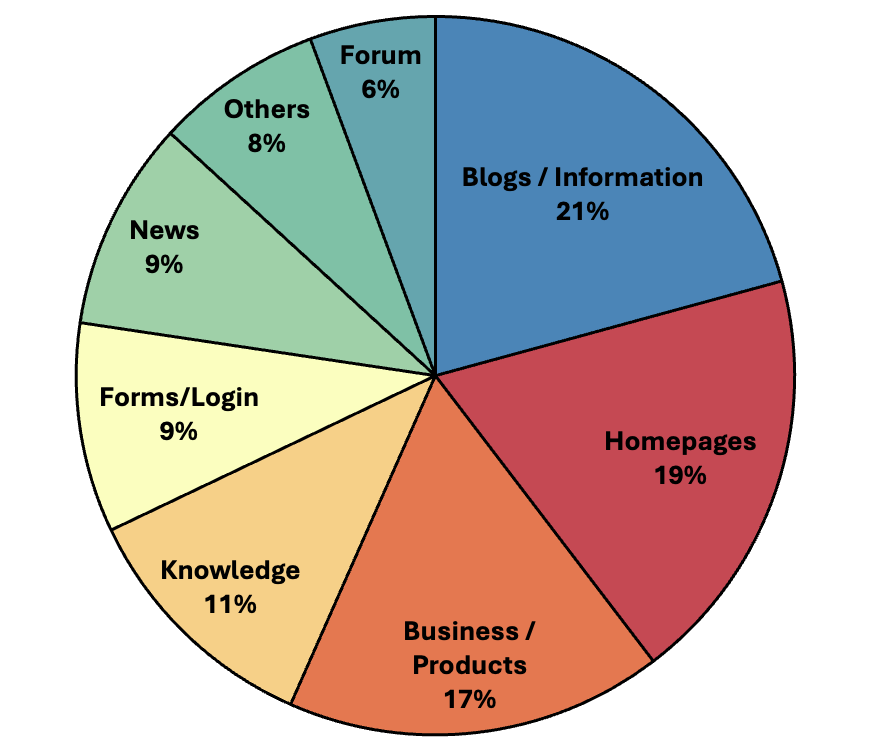
\includegraphics[width=0.3\textwidth]{figures/dataset_distribution.png}
  \caption{Distribution of Topics in Dataset}
  \label{fig:dataset_distribution}
\end{figure}

\subsection{Dataset Alignment}
Because Design2Code and Webcode2m use different strategies to purify 
their data, the datasets are harmonized before the analysis. 
The alignment contains (1) removing all external dependencies (e.g., images, audio, 
video, and external links) and substituting neutral placeholders (e.g., \texttt{src="placeholder.jpg"}
for images or \texttt{href="\#"} for links); (2) turning off executable content, 
such as scripts and other dynamic elements; (3) deleting non-visible content (e.g.,
advertisement-related tags or hidden elements) that are irrelevant in 
an image-to-code context and could otherwise possibly bias 
the accessibility metrics.



\section{Benchmarks}
The evaluation of the generated HTML/CSS is based on two complementary 
metrics: (1) Code Similarity and (2) Accessibility Metrics.

\subsection{Code Similarity}
Code similarity measures how closely the generated code matches the ground
truth reference. This is crucial for assessing the layout fidelity and 
semantic correctness. Following the metric defined in~\cite{si2024design2code}, 
the evaluation is based on a combination of high-level visual 
similarity and low-level element matching, which captures both 
structural and stylistic alignment. 
The metric contains five components:
text similarity (\(S_{\text{text}}\)), position similarity 
(\(S_{\text{pos}}\)), color difference (\(S_{\text{color}}\)), 
CLIP-based visual similarity (\(S_{\text{clip}}\)), 
and block size similarity (\(S_{\text{block}}\)). 
These scores collectively form the set 
\(\mathcal{S} = \{S_{\text{text}}, S_{\text{pos}}, S_{\text{color}}, S_{\text{clip}}, S_{\text{block}}\}\). 
The final score is computed as a weighted sum of these components:
\(
\textit{CodeSim} = \sum_{i=1}^{5} w_i \cdot S_i,
\),
where \(S_i \in \mathcal{S}\) denotes the \(i\)-th component score and \(w_i\) is its corresponding weight.
Following the findings of previous work, we adopt a uniform weighting for all components in this study, setting \(w_i = \frac{1}{5}\) for all \(i\).
The combination of those scores allows for a balanced view of the visual and 
structural similarity of the input and output.


\subsection{Accessibility Metrics}
Apart from counting violations, accessibility is evaluated along two
further dimensions: the relative quantity of violations and their 
severity. The combination of both metrics allows us to understand 
whether LLMs can decrease not only
the amount of accessibility violations but also their severity.\newline

\textbf{Inaccessibility Rate (IR):} Following prior
research~\parencite{alshayban2020accessibility}. It measures the 
percentage of DOM nodes with violations that exhibit at least one violation
relative to the number of nodes prone to such violations:
\begin{equation}
    \mathrm{IR} = \frac{N_{\mathrm{violations}}}{N_{\mathrm{total}}}
\end{equation}\newline

\textbf{Impact-Weighted Inaccessibility Rate (IWIR):}
To capture the severity according to the WCAG impact levels, IWIR
is introduced. Let $v_i$ denote the number of violations at impact 
level $i \in \{\text{minor}, \text{moderate}, \text{serious}, 
\text{critical}\}$ and let $w_i \in \{1,3,6,10\}$ be the corresponding 
weights. This scoring reflects the non-linear increase 
in impact for people with disabilities if a violation with a higher
impact occurs.
We normalize by the worst case for the observed counts:
\begin{equation}
  \mathrm{IWIR} = 
    \frac{\displaystyle\sum_{i=1}^{k} v_i \, w_i}
         {\displaystyle\sum_{i=1}^{k} v_i \, w_{\mathrm{max}}}
  \label{eq:iwir}
\end{equation}


% \begin{table}[ht]
% \centering
% \caption{Severity weights used in IWIR.}
%   \label{tab:weights}
%   \begin{tabular}{lcc}
%   \toprule
%   Impact level & WCAG level & Weight $w_i$ \\
%   \midrule
%   Minor    & AAA          & 1  \\
%   Moderate & AA or AAA    & 3  \\
%   Serious  & A or AA      & 6  \\
%   Critical & A          & 10 \\
%   \bottomrule
%   \end{tabular}
% \end{table}





